
% Component-and-Connector styles

%1
\newcommand{\qComponentAndConnectorOne}{
\begin{ClosedQuestion}
	Consider the Service-Oriented Architecture architectural style
		
    \optionA{The main quality this style addresses is interoperability.}
    \optionB{It cannot be applied when the system includes legacy systems.}
    \optionC{Its enterprise service bus cannot support asynchronous communication between the components.}
    \optionD{The typical communication pattern is point-to-point.}
 \putOptions 
\end{ClosedQuestion}
}

%2
\newcommand{\qComponentAndConnectorTwo}{
\begin{ClosedQuestion}
	Consider the following view of the Adventure Builder system
	
	\begin{center}
		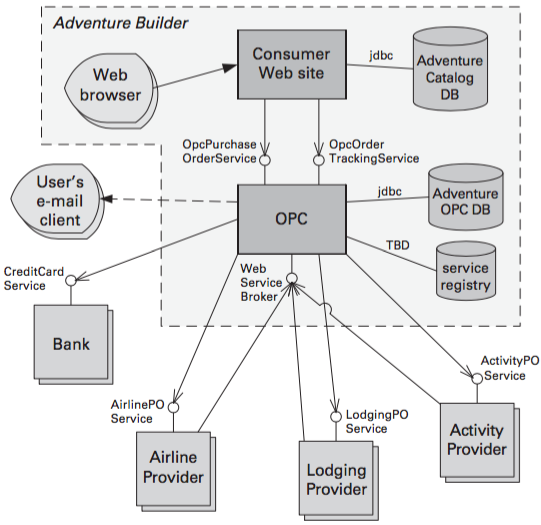
\includegraphics[width=80mm]{AdventureBuilder-SOA}
	\end{center}
	
	In this view the following architectural styles are used
	
		
    \optionA{Service-oriented architecture, and Client-server.}
    \optionB{Service-oriented architecture, and Shared-data.}
    \optionC{Service-oriented architecture, Shared-data, and Peer-to-peer.}
    \optionD{Service-oriented architecture, Shared-data, Peer-to-peer, and Client-server.}
 \putOptions 
\end{ClosedQuestion}
}
	
%3
\newcommand{\qComponentAndConnectorThree}{
\begin{ClosedQuestion}
	Consider the following view of the Adventure Builder system
	
	\begin{center}
		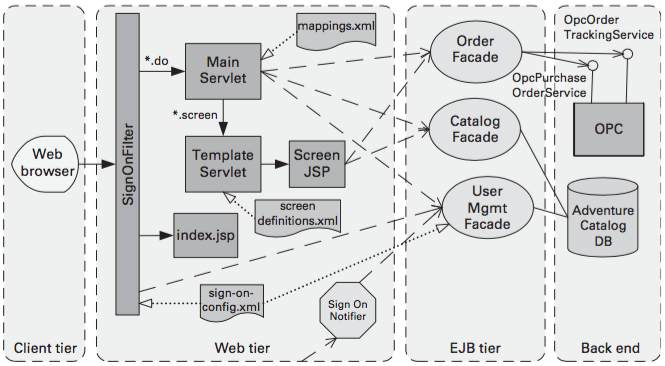
\includegraphics[width=100mm]{AdventureBuilder-Tiers}
	\end{center}
	
	In this view the following architectural styles are used
		
    \optionA{Tiers.}
    \optionB{Tiers, and Shared-data.}
    \optionC{Tiers, Shared-data, and Service-oriented architecture.}
    \optionD{Tiers, Shared-data, Service-oriented architecture, and Client-server.}
 \putOptions 
\end{ClosedQuestion}
}

% Allocation viewtype

%4
\newcommand{\qAllocationOne}{
\begin{ClosedQuestion}
	Consider the work assignment architectural style of the allocation viewtype.
			
    \optionA{It assigns components and connectors to people and teams.}
    \optionB{It is useful for the project managers.}
    \optionC{It does not consider the software that is outsourced.}
    \optionD{It allows to estimate the cost of hardware.}
 \putOptions 
\end{ClosedQuestion}
}

%5
\newcommand{\qAllocationTwo}{
\begin{ClosedQuestion}
	Consider the deployment architectural style of the allocation viewtype.
			
    \optionA{It assigns modules to the hardware.}
    \optionB{It cannot assign software elements to virtual servers because they are not hardware.}
    \optionC{For each set of software elements there is a single possible assignment to hardwre.}
    \optionD{It is useful for system administrators.}
 \putOptions 
\end{ClosedQuestion}
}

%6
\newcommand{\qAllocationThree}{
\begin{ClosedQuestion}
	Consider the install architectural style of the allocation viewtype.
			
    \optionA{The development team is the main stakeholder interesting in these views.}
    \optionB{It assigns modules to files.}
    \optionC{It is completely independent of the deployment architectural style.}
    \optionD{It helps on the configuration of systems.}
 \putOptions 
\end{ClosedQuestion}
}

% Infinispan views

%7
\newcommand{\qInfinispanOne}{
\begin{ClosedQuestion}
	Consider the Infinispan system when it is configured as a remote data grid. The relation between the Applications and the Grid is
			
    \optionA{Client-server.}
    \optionB{Peer-to-peer.}
    \optionC{Master-slave.}
    \optionD{Pipe-and-filter.}
 \putOptions 
\end{ClosedQuestion}
}

%8
\newcommand{\qInfinispanTwo}{
\begin{ClosedQuestion}
	In the description of Infinispan system can be read
	
	\begin{quote}
		Infinispan supports several pluggable cache stores-adapters that can be used to persist data to disk or any form of secondary storage. The current default implementation is a simplistic hash bucket and linked list implementation, where each hash bucket is represented by a file on the filesystem. While easy to use and configure, this isn't the best-performing implementation.
	\end{quote}
	
	The architectural style(s) that should be used to illustrate the sentence is (are)
			
    \optionA{Decomposition.}
    \optionB{Generalization.}
    \optionC{Decomposition and Generalization.}
    \optionD{Peer-to-peer.}
 \putOptions 
\end{ClosedQuestion}
}

%9
\newcommand{\qInfinispanThree}{
\begin{ClosedQuestion}
	In the description of Infinispan system can be read
	
	\begin{quote}
		When dealing with thread pools to process such asynchronous tasks, there is always a context switching overhead. That threads are not cheap resources is also noteworthy. Allocating appropriately sized and configured thread pools is important to any installation making use of any of the asynchronous features of Infinispan.
	\end{quote}
	
	The architectural style that should be used to illustrate the sentence is
			
    \optionA{Client-server.}
    \optionB{Communicating processes.}
    \optionC{Peer-to-peer.}
    \optionD{Shared-data.}
 \putOptions 
\end{ClosedQuestion}
}

% Micro-services and Amazon Cloud

%10
\newcommand{\qMicroAndAmazonOne}{
\begin{ClosedQuestion}
	Consider the following distinction between Monoliths and Microservices made by Matin Fowler
	
	\begin{center}
		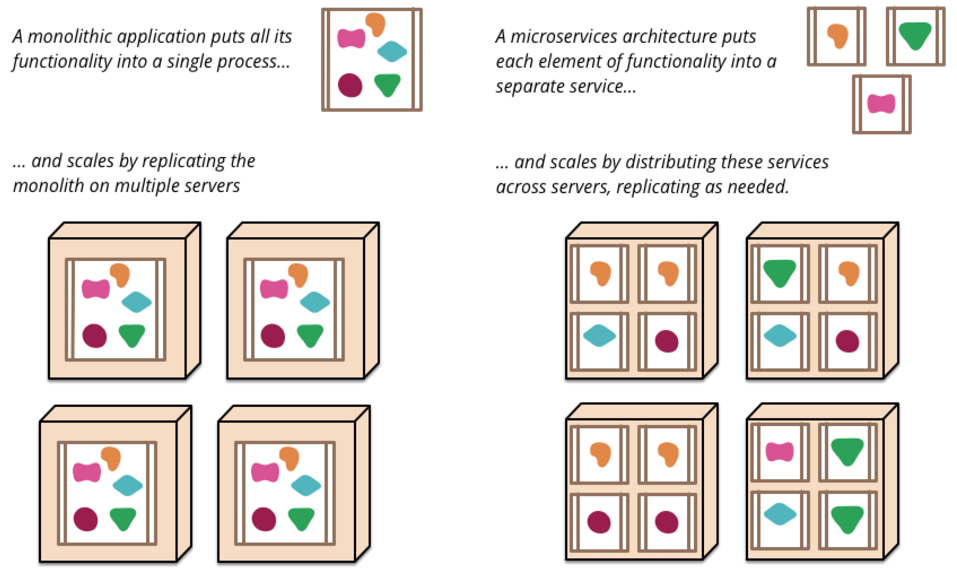
\includegraphics[width=100mm]{MonolithsVsMicroservices}
	\end{center}
	
	If we try to map this figure into a set of views we will need.
			
    \optionA{A decomposition view.}
    \optionB{A view of the component-and-connector viewtype.}
    \optionC{A view of the component-and-connector viewtype and a deployment view.}
    \optionD{A decomposition view, a view of the component-and-connector viewtype and a deployment view.}
 \putOptions 
\end{ClosedQuestion}
}

%11
\newcommand{\qMicroAndAmazonTwo}{
\begin{ClosedQuestion}
	Consider the following representation of Amazon's architecture (sorry for the figure's layout: \textbf{save trees})
			
	\begin{center}
		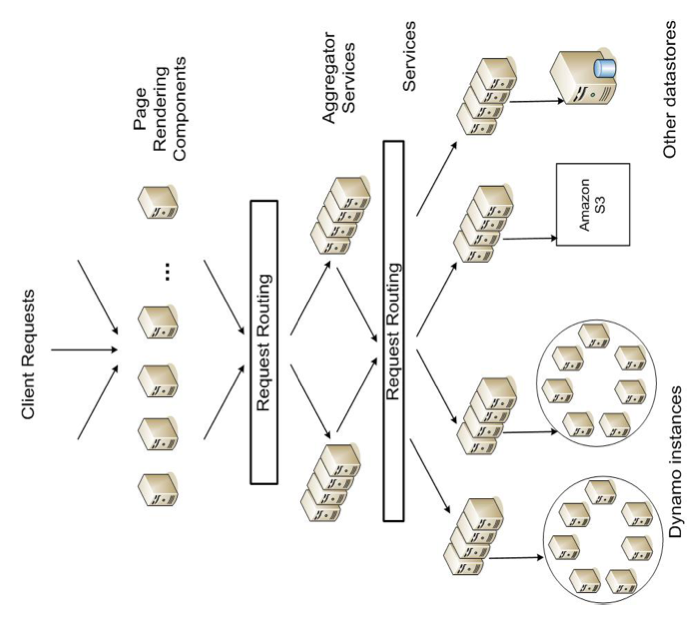
\includegraphics[width=80mm]{AmazonArchitecture}
	\end{center}
	
	What is the most relevant architecture style that is used in this figure?
	
    \optionA{Client-server to represent performance.}
    \optionB{Tiers to represent scalability.}
    \optionC{Service-oriented architecture to represent interoperability.}
    \optionD{Shared-data to represent modifiability.}
 \putOptions 
\end{ClosedQuestion}
}

%12
\newcommand{\qMicroAndAmazonThree}{
\begin{ClosedQuestion}
	In the interview Werner Vogels from Amazon gives to Jim Gray, Werner Vogels says that
	
	\begin{quote}
		The stored data formats are decoupled from the format in which you communicate data items. If there is no need for sharing schemas of the actual storage layout, you can focus on making sure that the service interfaces can evolve in a way that allows you to handle variations of data formats. 
	\end{quote}
	
	Which means that in the software architecture of Amazon's systems
			
    \optionA{The data-shared architectural style is not applied because data is encapsulated inside services.}
    \optionB{The sharing of data is done using a service-oriented architecture.}
    \optionC{Modifiability is not a concern of their architecture.}
    \optionD{The decouple of data formats does not support scalability because of the transactional properties.}
 \putOptions 
\end{ClosedQuestion}
}

% Jenkings views

%13
\newcommand{\qJenkinsOne}{
\begin{ClosedQuestion}
	Consider the following representation of the Buildbot system.
	
	\begin{center}
		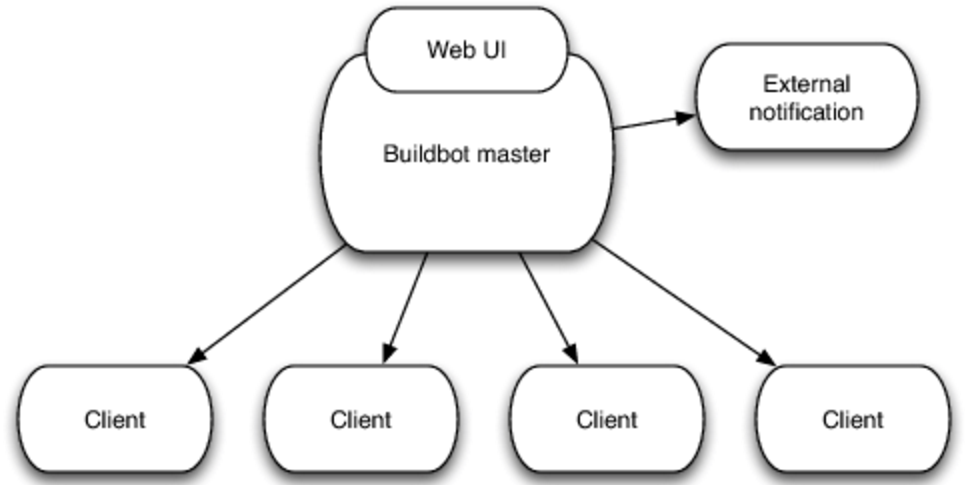
\includegraphics[width=80mm]{BuildbotArchitecture}
	\end{center}
	
	The architecture style between the Buildbot Master and the Clients is:
			
    \optionA{Peer-to-peer.}
    \optionB{Shared-data where the Buildbot is the data accessor.}
    \optionC{Client-server where the Buildbot is the client.}
    \optionD{Client-server where the Buildbot is the server.}
 \putOptions 
\end{ClosedQuestion}
}

%14
\newcommand{\qJenkinsTwo}{
\begin{ClosedQuestion}
	In the Continuous Integration case can be read
	\begin{quote}
		Build notification: The outcomes of builds generally need to be communicated to interested clients, either via pull (Web, RSS, RPC, etc.) or push notification (e-mail, Twitter, etc.) This can include notification of all builds, or only failed builds, or builds that haven't been executed within a certain period.
	\end{quote}
		The architectural style used in push notifications is
			
    \optionA{Publish-subscribe.}
    \optionB{Client-server.}
    \optionC{Shared-date.}
    \optionD{Generalization.}
 \putOptions 
\end{ClosedQuestion}
}

%15
\newcommand{\qJenkinsThree}{
\begin{ClosedQuestion}
	Consider the following representation of the CDash system
	
	\begin{center}
		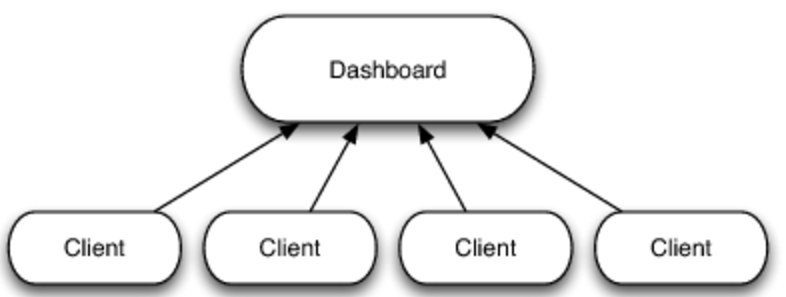
\includegraphics[width=80mm]{DashArchitecture}
	\end{center}
	
	The architecture style between the Dashboard and the Clients is:
			
    \optionA{Peer-to-peer.}
    \optionB{Shared-data where the Dashboard is the repository.}
    \optionC{Client-server where the Dashboard is the client.}
    \optionD{Client-server where the Dashboard is the server.}
 \putOptions 
\end{ClosedQuestion}
}
